\chapter[Reconstrução da Física do Canal eGamma do Experimento ATLAS]
{Reconstrução da Física do Canal e/$\gamma$ do Experimento ATLAS}
\label{cap:reco}

A alta energia e luminosidade do \gls{lhc} (Seção~\ref{sec:lhc}) oferecem um alto alcance para
explorar física, desde a medição precisa de propriedades de objetos conhecidos, a
ultrapassar a fronteira de energias onde a física ainda não havia sido experimentada.
Por ser um detector de propósito geral, o \gls{atlas} (Seção~\ref{sec:ATLAS}), deve ser capaz de
explorar diversos dos objetivos do \gls{lhc} (Subseção~\ref{ssec:obj_lhc}), e
para isso ele precisar ter a capacidade de explorar um largo espectro de assinaturas
físicas. Esse fato guiou a otimização do projeto do \gls{atlas}, dando as especificações de sensibilidade e precisão do
detector para que seja possível através das assinaturas realizar a reconstrução
com precisão da física ocorrida nas colisões. O foco principal é na busca pelo
bóssom de Higgs \cite{ATLAS_TDR2}, com o objetivo de provar a origem da escala
eletrofraca\footnote{A escala eletrofraca existe somente no estado primitivo descrito na
Subseção~\ref{ssec:bossoms}.}. 

A física se apoia em algoritmos
para realizar a busca pelas assinaturas, sendo este capítulo dedicado aos
algoritmos que fazem a reconstrução do Canal \gls{eg},
onde se deseja encontrar as assinaturas dessas partículas (e dos pósitrons, que
tem a mesma assinatura de elétrons, excluindo a direção de deflexão de seus
traços, oposta àquela de elétrons devido a sua carga positiva). A identificação
dessas partículas é de fundamental importância por formarem os canais de
decaimentos mais limpos do bóssom de Higgs (Sessão~\ref{sec:busca_higgs}). Além
disso, outras partículas como o bóssom Z e partícula $\text{J}/\Psi$, podem ser
utilizadas para melhorar a escala de medida de energia dos calorímetros e
estudar sua linearidade de resposta por terem suas massas bem conhecidas, 
em especial os decaimentos de elétrons do
$\text{J}/\Psi$ para baixas energias ($\gls{Et} > 5$ GeV), onde se esperam encontrar 
decaimentos leptônicos do bóssom de Higgs de menor energia ($\gls{Et} > 7$ GeV).
Outras assinaturas experimentais são as de hádrons e jatos, que serão tratadas
quando abordando o Canal \gls{eg}, por serem o ruído de fundo do qual se deseja
filtrar nesse canal. Entretanto existem setores de física que se
interessam por esses decaimentos, como o já citado decaimento do bóssom W em jatos
duplos\footnote{A citação foi realizada no Subtópico~\ref{par:cal_part_id}.}. 
Além disso, múons constituem de outras assinaturas, uma vez que interagem
pouco com os calorímetros, tendo seu próprio subsistema, o Espectômetro de
Múons. Existem outras três assinaturas:
táons, sabores pesados e léptons neutrinos. Os táons decaem
rapidamente em múons (ou elétrons) e mais dois neutrinos, ou ainda, em um ou três
píons carregados, de forma que sua assinatura é
feita nos espectometros de múons (ou calorímetro), ou de chuveiros \gls{had} com um ou três
traços isolados apontando para o chuveiro. Os sabores pesados procuram
assinaturas de mésons pesados, que geralmente decaem a menos de 1 mm do ponto de
colisão, sendo necessário criar um vértice secundário que será identificado com
a alta precisão do Detector de Pixel. Finalmente, léptons neutrinos escapam da
deteção, para sua assinatura é utilizada a propriedade de conservação de
\gls{pt}, de modo que, quando há quantidade suficiente de \gls{ptmiss}, há indicios
de que algo escapou do processo de deteção.

Os algoritmos são implementados em dois ambientes diferentes, um ambiente mais
restrito, necessário devido ao alto nível de ruído físico gerado nas condições 
impostas do \gls{lhc} (citadas no Tópico~\ref{sssec:minb_ue_pileup}): o
\glsdesc{sf} (Seção~\ref{sec:sf}). Nesse ambiente o tempo de discriminação 
é limitado a latência suportada pela capacidade computacional das máquinas localizadas 
no \gls{ip}1. O trabalho segue com o desenvolvimento do algoritmo HLT\_EgammaCaloRinger 
(Subseção~\ref{ssec:hlt_ringer}), um algoritmo alternativo proposto para o
Segundo Nível de Filtragem desse sistema. A versão implementada pela colaboração, o T2Calo (Subseção~\ref{ssec:t2calo}), 
também é descrita em detalhes. Por sua vez o outro ambiente, o \glsdesc{sr}
(Seção~\ref{sec:sr}), visa fazer uma análise mais precisa dos eventos de colisão e da 
física gerada, sendo o \glsdesc{sf}, nos níveis mais altos de filtragem, 
nada mais que uma versão restringida baseada no mesmo. Para que a Colaboração tenha 
um melhor contato com o algoritmo proposto e entenda o seu funcionamento, se fez
necessário a implementação (Tópico~\ref{sssec:egringer_impl}) de uma versão no Sistema 
de \glsdesc{sr} (Subseção~\ref{ssec:egringer}) para que os físicos o utilizassem nas suas 
análises a posteriori. A versão padrão (Subseção~\ref{ssec:egamma}) utilizada
pelos físicos também foi abordada.


\section{Busca pelo bóssom de Higgs}
\label{sec:busca_higgs}

\newacronym[type=Abrev]{mh}{\ensuremath{m_H}}{massa do bóssom de Higgs} 
\newacronym[type=Abrev]{lep}{LEP}{\emph{Large Electron Positron Collider}} 
\glsunset{mh}

O bóssom de Higgs no setor do \gls{mp} é amplamente irrestrito, de forma que sua
massa, \acrshort{mh}, não é prevista pela teoria. Um limite superior na ordem de
$\sim$1 TeV teórico, e um limite inferior experimental\footnote{As exclusões
citadas foram feitas para um nível de confiança de 95\%.\label{fn:95cl}} de 95,2
GeV \cite{lep_higgs_1999} por um experimento anterior do \gls{cern}, o \gls{lep}, determinam a região para a qual
se esperava encontrar o bóssom de Higgs durante a época das últimas propostas técnicas
do projeto do \gls{atlas} \cite{ATLAS_TDR,ATLAS_TDR2}, por volta de 1999. 

Um estudo do potêncial de descoberta do bóssom de Higgs através de seus
possíveis canais de decaimentos explorados pelo programa de física do
\gls{atlas} foi revisado na propostas citadas. Esses canais são:

\begin{itemize}
\item $H\rightarrow\gamma\gamma$ (110 a 150 GeV/$c^2$), produção direta;
\item $H\rightarrow\gamma\gamma$ (110 a 150 GeV/$c^2$), da produção associada $WH$, $ZH$ e
$t\bar{t}H$, usando um lépton (e, $\mu$) rotulado do decaimento dos bóssom W, Z ou
do quark \emph{top};
\item $H\rightarrow b\bar{b}$ (110 a 130 GeV/$c^2$), da produção associada $WH$, $ZH$ e
$t\bar{t}H$, usando um lépton (e, $\mu$) rotulado do decaimento dos bóssom W, Z ou
do quark \emph{top};
\item $H\rightarrow ZZ^*\rightarrow4l$ (110 a 600 GeV/$c^2$. O símbolo $^*$ representa uma partícula 
que está fora de sua fronteira de massa\footnote {Na literatura em inglês 
\emph{off the mass shell}, ou simplesmente \emph{off
shell}.} na relação massa-momento dada pela equação~\ref{eq:rel_mom}. Essas
partículas só existem como estados intermediários, constituindo partículas
virtuais, e estão de acordo com o princípio da incerteza, em que as partículas
só podem existir nesse estado durante um tempo menor que uma fração da
constante 
de Plank pela diferença de energia, ou $\Delta E \Delta t \gtrsim h$), onde l
representa estes léptons: $e,\mu$; 
\item $H\rightarrow ZZ\rightarrow4l$ e $H\rightarrow ZZ\rightarrow ll\nu\nu$i
(200 a 600 GeV/$c^2$), aqui $\nu$ são os léptons neutrinos;
\item $H\rightarrow WW\rightarrow l\nu jj$ e $H\rightarrow ZZ\rightarrow ll jj$
($\sim$600 a 1 TeV),
onde $jj$ representa o decaimento em jatos duplos;
\item $H\rightarrow WW^*\rightarrow l\nu l\nu$ (110 a 300 GeV/$c^2$). 
\end{itemize}


Nesse estudo se utilizou simulações
de Monte Carlo do \emph{Pythia}, através da significância desses 
canais numa região de 80-1000 GeV/$c^2$ (lembrando que na época só havia sido excluído
o bóssom de Higgs para \gls{mh} < 95,2), utilizando os valores de resposta dos
subdectores, resolução e capacidade esperadas de identificação de sinais e rejeição 
de ruídos redutivéis. 
Os resultados desse estudo estão resumidos na Figura~\ref{fig:higgs_sim_atlas},
mostrando a significância do sinal para uma luminosidade integrada\footnote{A 
luminosidade integrada, como seu nome indica, não passa da integral da luminosidade 
instantânea no tempo de operação do \gls{lhc}: $\int{L_{inst} dt}$.} de
100 $\text{fb}^{-1}$. Para efeito de comparação na
Figura~\ref{fig:higgs_branch_ratio} há as relações entre os canais
e seus alcânces em massa. A Figura~\ref{fig:higgs_production} contêm a seção
de choque esperada para as possíveis massas.

\begin{figure}[ht!]
    \label{fig:higgs_expected}
    \begin{center}
%
        \subfigure[]{%
            \label{fig:higgs_branch_ratio}
            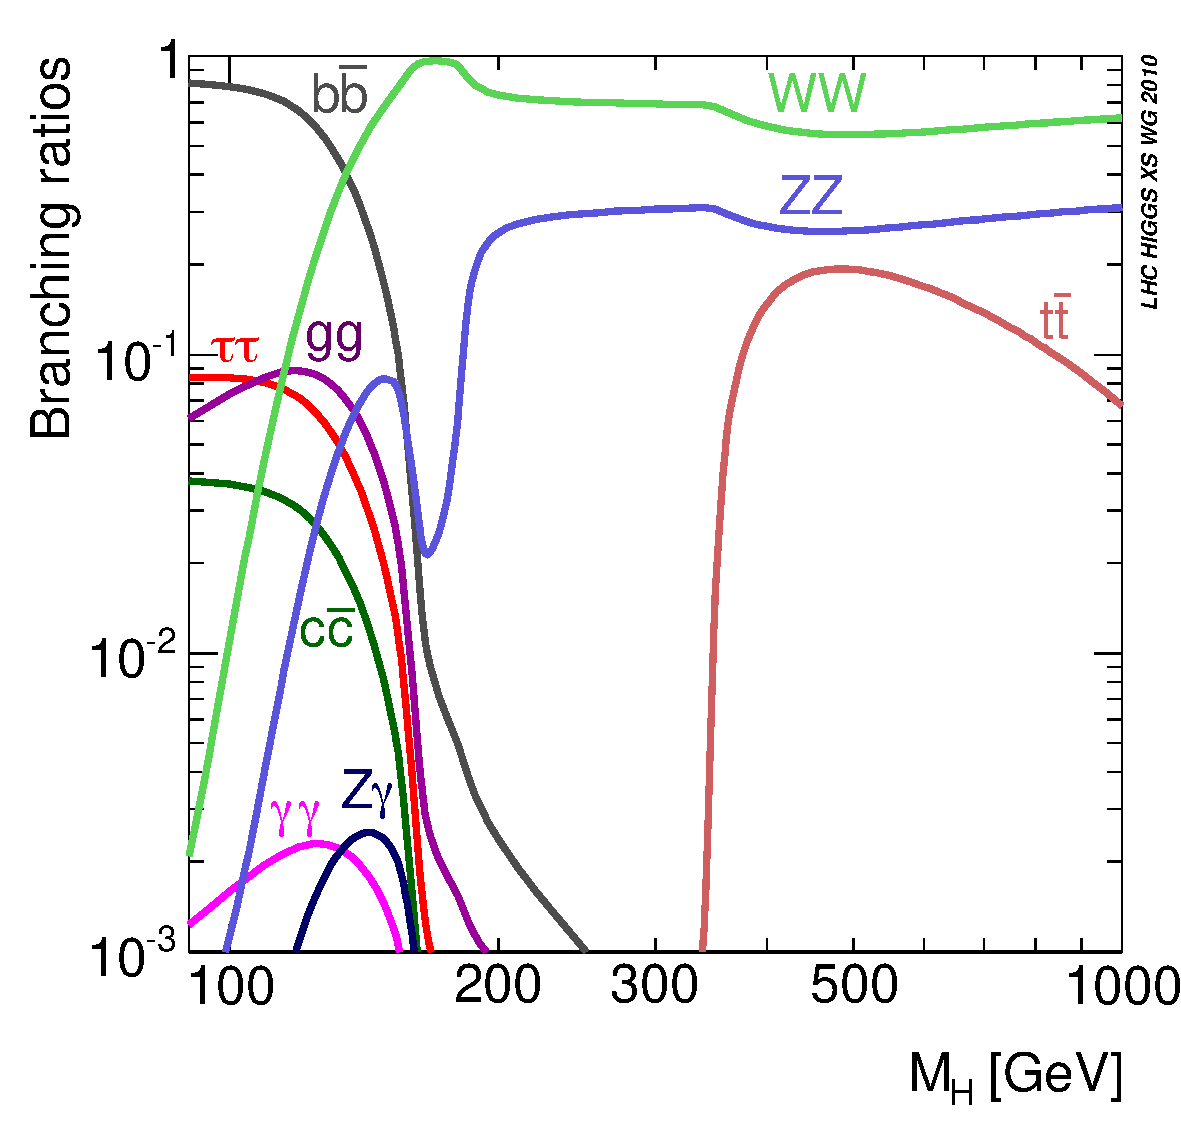
\includegraphics[width=0.47\textwidth,height=6cm]{imagens/higgs_branch_ratio.pdf}
        }%\hspace{0.1\textwidth}
        \subfigure[]{
            \label{fig:higgs_production}
            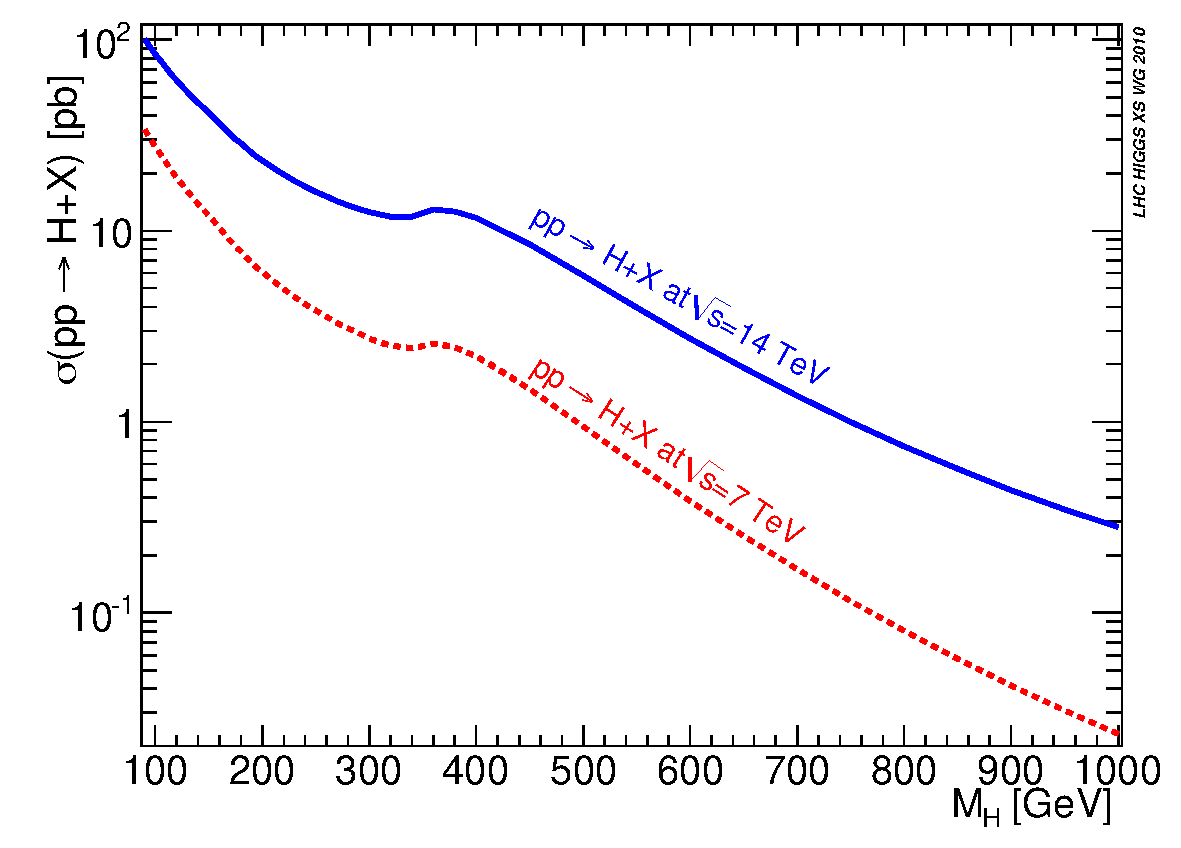
\includegraphics[width=0.47\textwidth,height=6cm]{imagens/higgs_production.pdf}
        }\\
        \subfigure[]{%
            \label{fig:higgs_sim_atlas}
            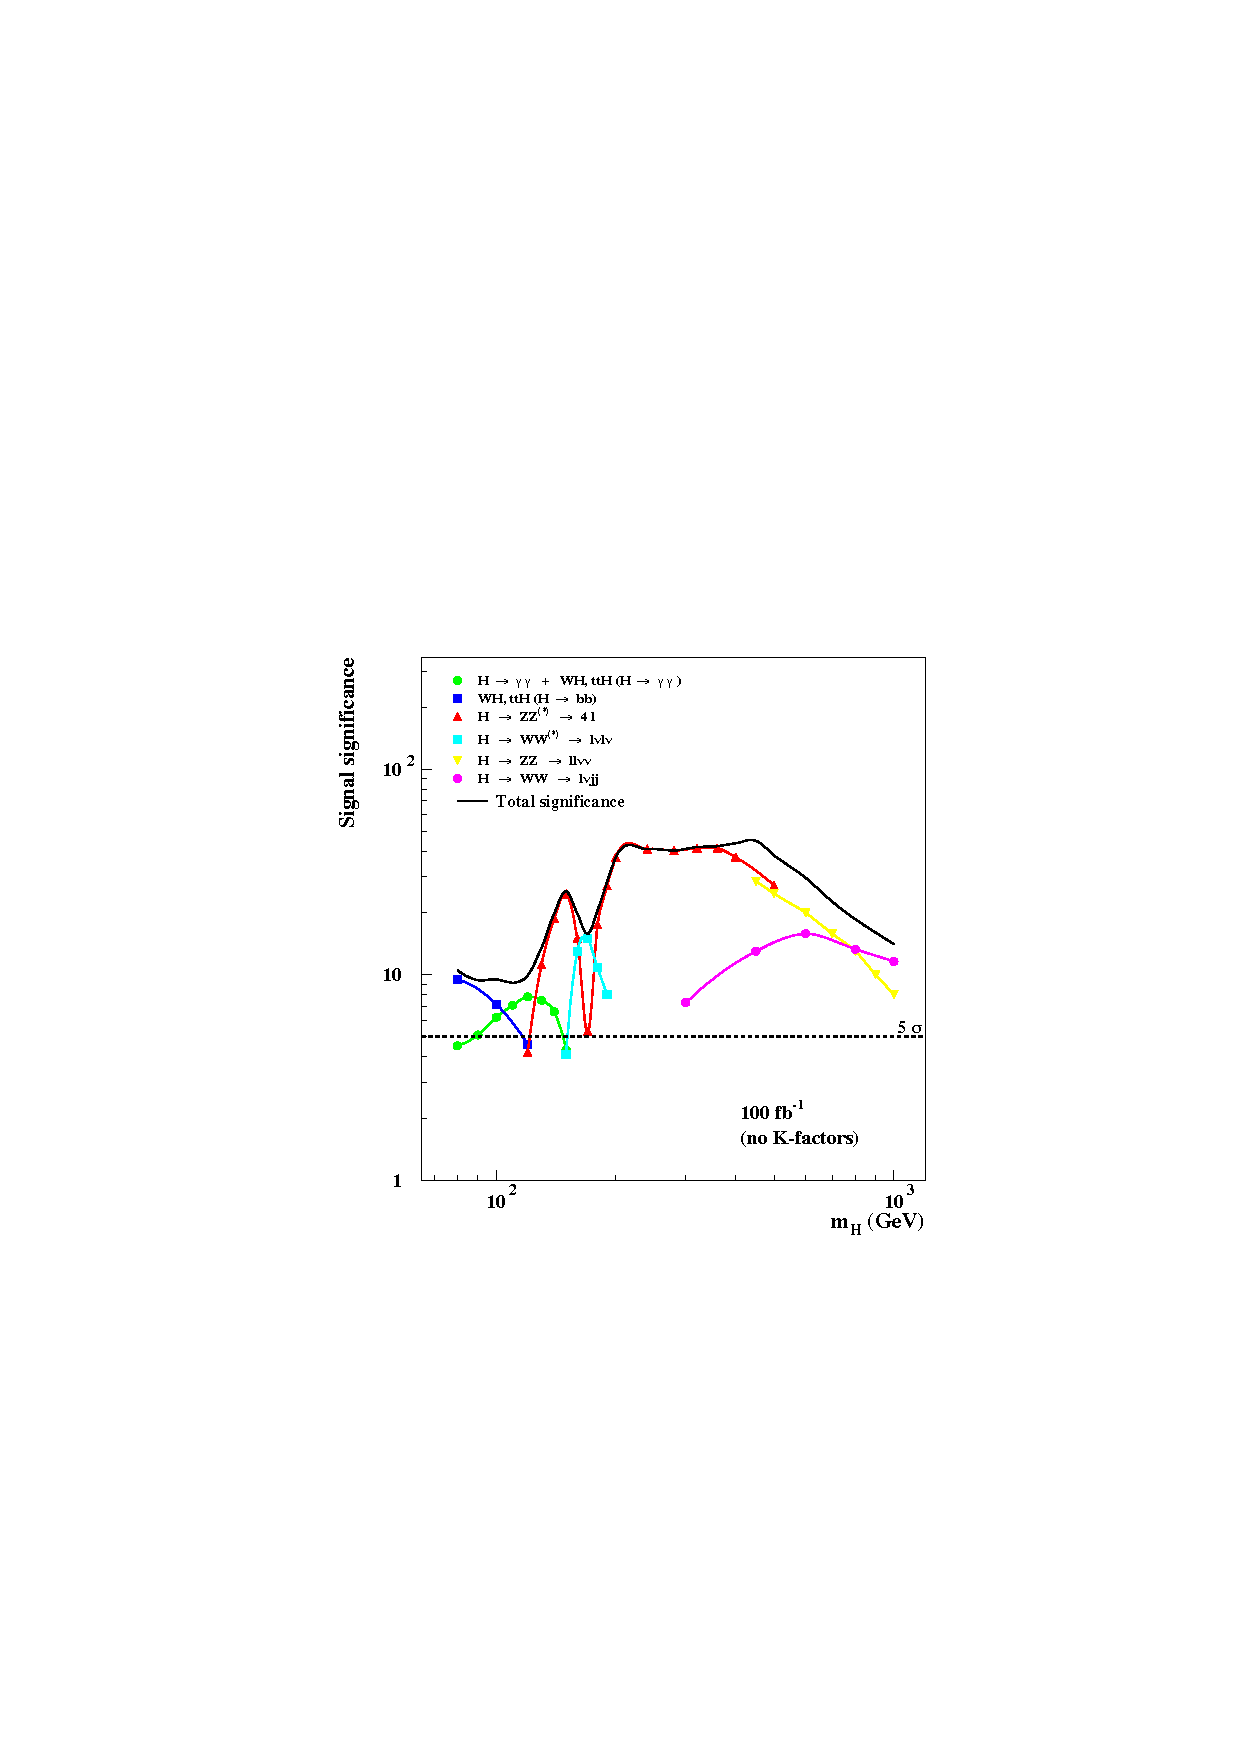
\includegraphics[width=.6\textwidth]{imagens/higgs_sim_atlas.pdf}
        }
    \end{center}
\caption[Simulação da significância dos canais de decaimento do bóssom
de Higgs explorados pelos ATLAS, as relações de seus canais e alcances em massa,
e a seção de choque do mesmo.]
{Os decaimentos do bóssom de Higgs do MP e suas relações de
seus canais e alcances em massa,~\ref{fig:higgs_branch_ratio}, e os seus valores de seção de choque para suas
repectivas massas,~\ref{fig:higgs_production}, ambos extraídas de \cite{lhc_higgs_group}. 
Em \ref{fig:higgs_sim_atlas} está uma simulação da significancia dos possíveis canais de decaimento do
bóssom de Higgs, explorados pelo ATLAS, para uma luminosidade integrada de
$100fb^{-1}$, utilizando as eficiências esperadas para a deteção das
assinaturas dos estados finais e resoluções dos subdetectores, extraído de
\cite{ATLAS_TDR2}.}
\end{figure}

Observe que decaimentos do bóssom de Higgs mais frequentes não são,
necessariamente, os canais com melhor significância esperada. Aqueles canais em
que se tem mais facilidade de observar os decaimentos finais e poder associá-los
a produção de um bóssom de Higgs podem ter mais significância do que canais com
maior produção para uma dada massa. Isso reflete, por outro lado, na importância
dos algoritmos de reconstrução, obtendo melhor eficiência na reconstrução dos
estados finais facilitariam a encontrar o bóssom com menor quantidade de dados.
Os canais mais importantes nas regiões de massa intermediária, $\gls{mh}<2m_Z$,
onde se espera que os decaimentos reconstruam um pico de massa, são 
o canal de quatro léptons, $H\rightarrow ZZ^* \rightarrow 4l$, o canal de
produção direta em dois fótons, $H\rightarrow \gamma\gamma$, junto com os
canais de produção associada com o mesmo estados finais, . Para massas por volta
de 170 GeV/$c^2$, onde a produção de $ZZ^*$ é suprimida, o potêncial da descoberta do
Higgs pode ser elevada pelo decaimento $H\rightarrow WW^*\rightarrow l\nu l\nu$,
nesse caso, o sinal deverá ser observado como um excesso de eventos. O canal de
quatro léptons com dois bóssoms Z reais é o dominante na região de
$\gls{mh}>2m_Z$, cobrindo uma vasta região de massa\footnote{Por isso chegou a
ser referênciado como canal banhado a ouro.}. Em massas mais elevadas, por volta de 600 GeV/$c^2$ até 1
TeV, outros canais como $H\rightarrow WW\rightarrow l\nu jj$, $H\rightarrow
WW\rightarrow ll\nu\nu$ são utilizados para a busca do bóssom de Higgs.

Posteriormente, outro canal foi adicionado, por outros estudos
\cite{atlas_tautau,atlas_tautau2}:

\begin{itemize} 
\item $H\rightarrow \tau \tau \rightarrow ll4\nu$ e $H\rightarrow \tau \tau
\rightarrow l\tau_{had}3\nu$ (110 a 150 GeV/$c^2$), onde $\tau_{had}$ seria o
decaimento do táon em píons especificados no início deste capítulo.
\end{itemize} 

Assim, a reconstrução de elétrons e múons fazem parte de grande
parte dos canais explorados para a vasta região de massa em que se espera
encontrar o bóssom de Higgs, inclusive um dos canais
mais importante por cobrir uma vasta região de massa. Se o Higgs existir com
uma massa mais baixa, os fótons serão necessários para poder encontrar o bóssom,
mostrando a importância do Canal \gls{eg}. 

\begin{figure}[t!]
    \label{fig:higgs_exclusion}
    \begin{center}
    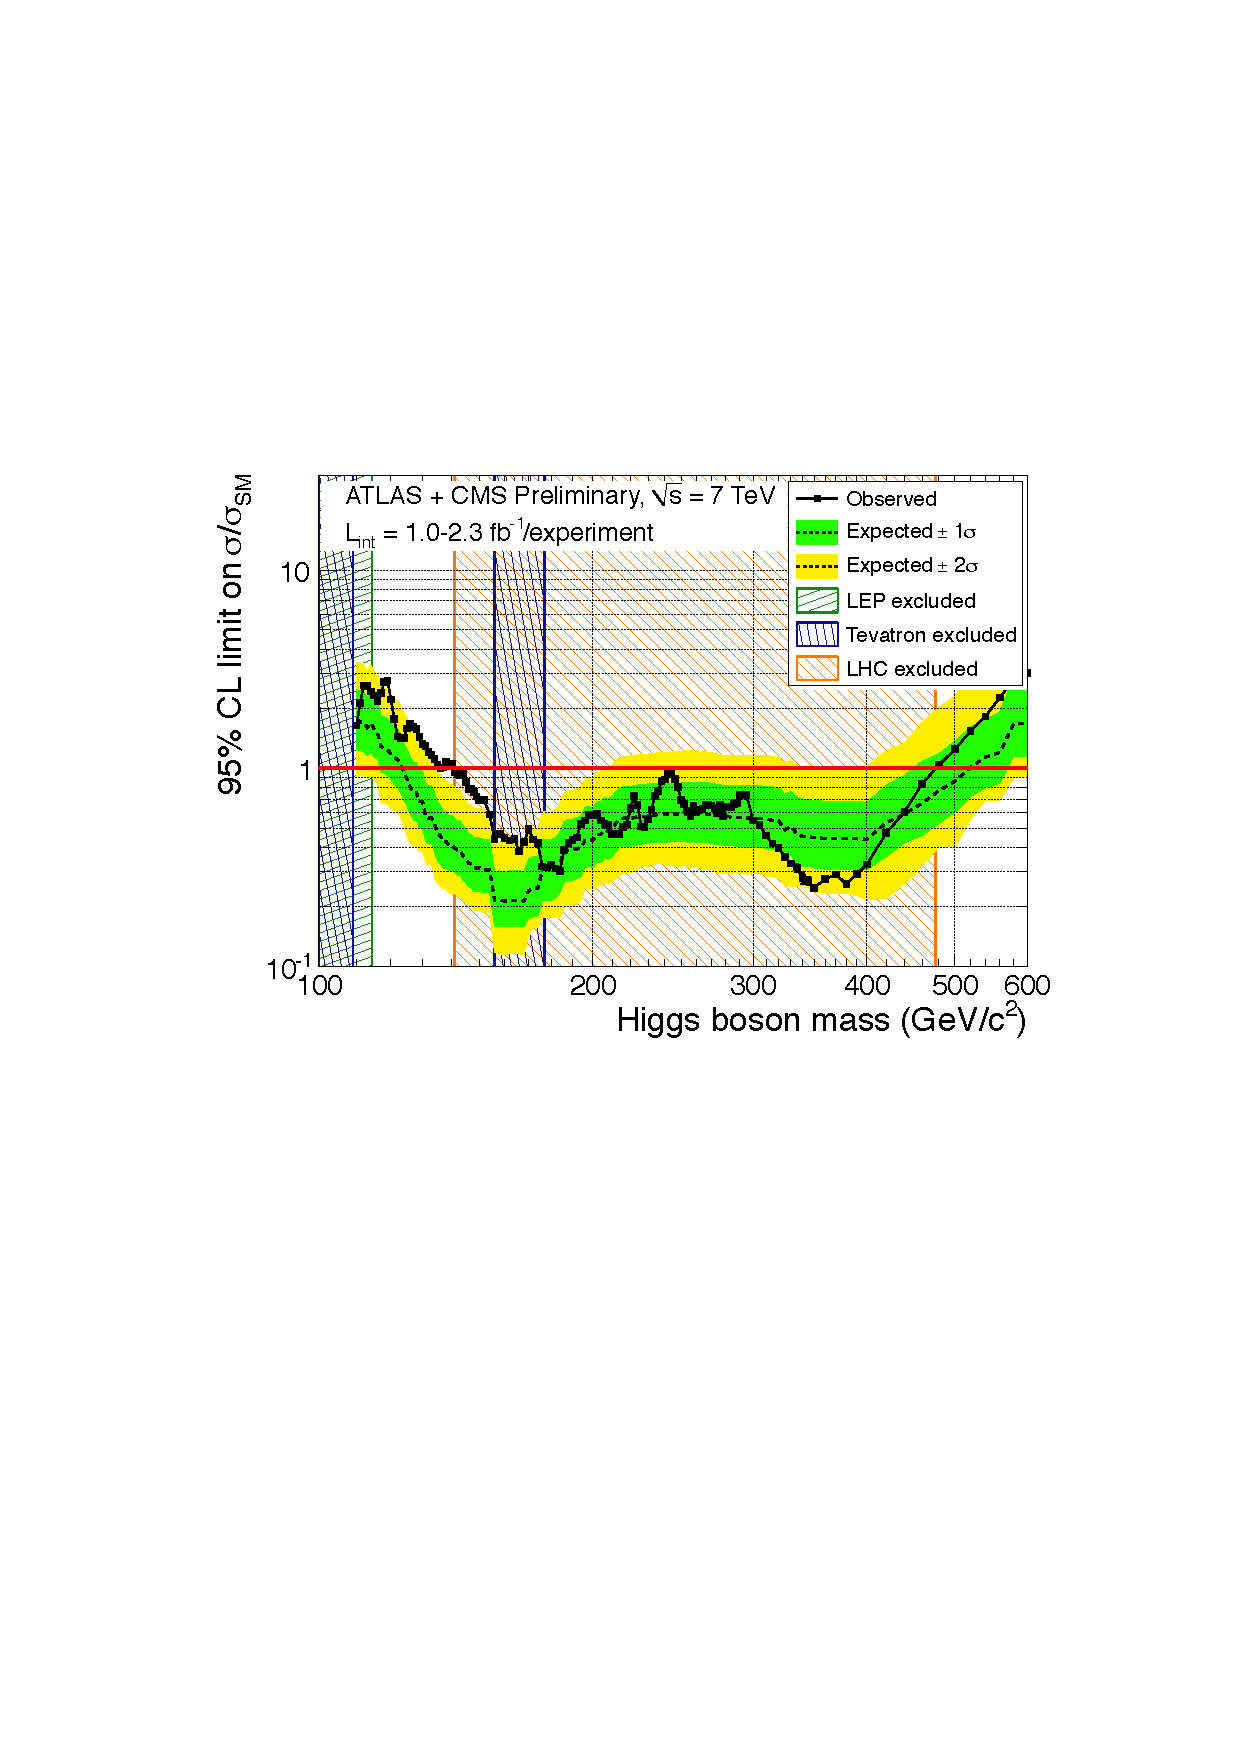
\includegraphics[width=0.8\textwidth]{imagens/exclusion_cms_atlas.pdf}
%
%        \subfigure[LEP, extraído de \cite{lep_higgs_2008}.]{%
%            \label{fig:lep_exclusion}
%            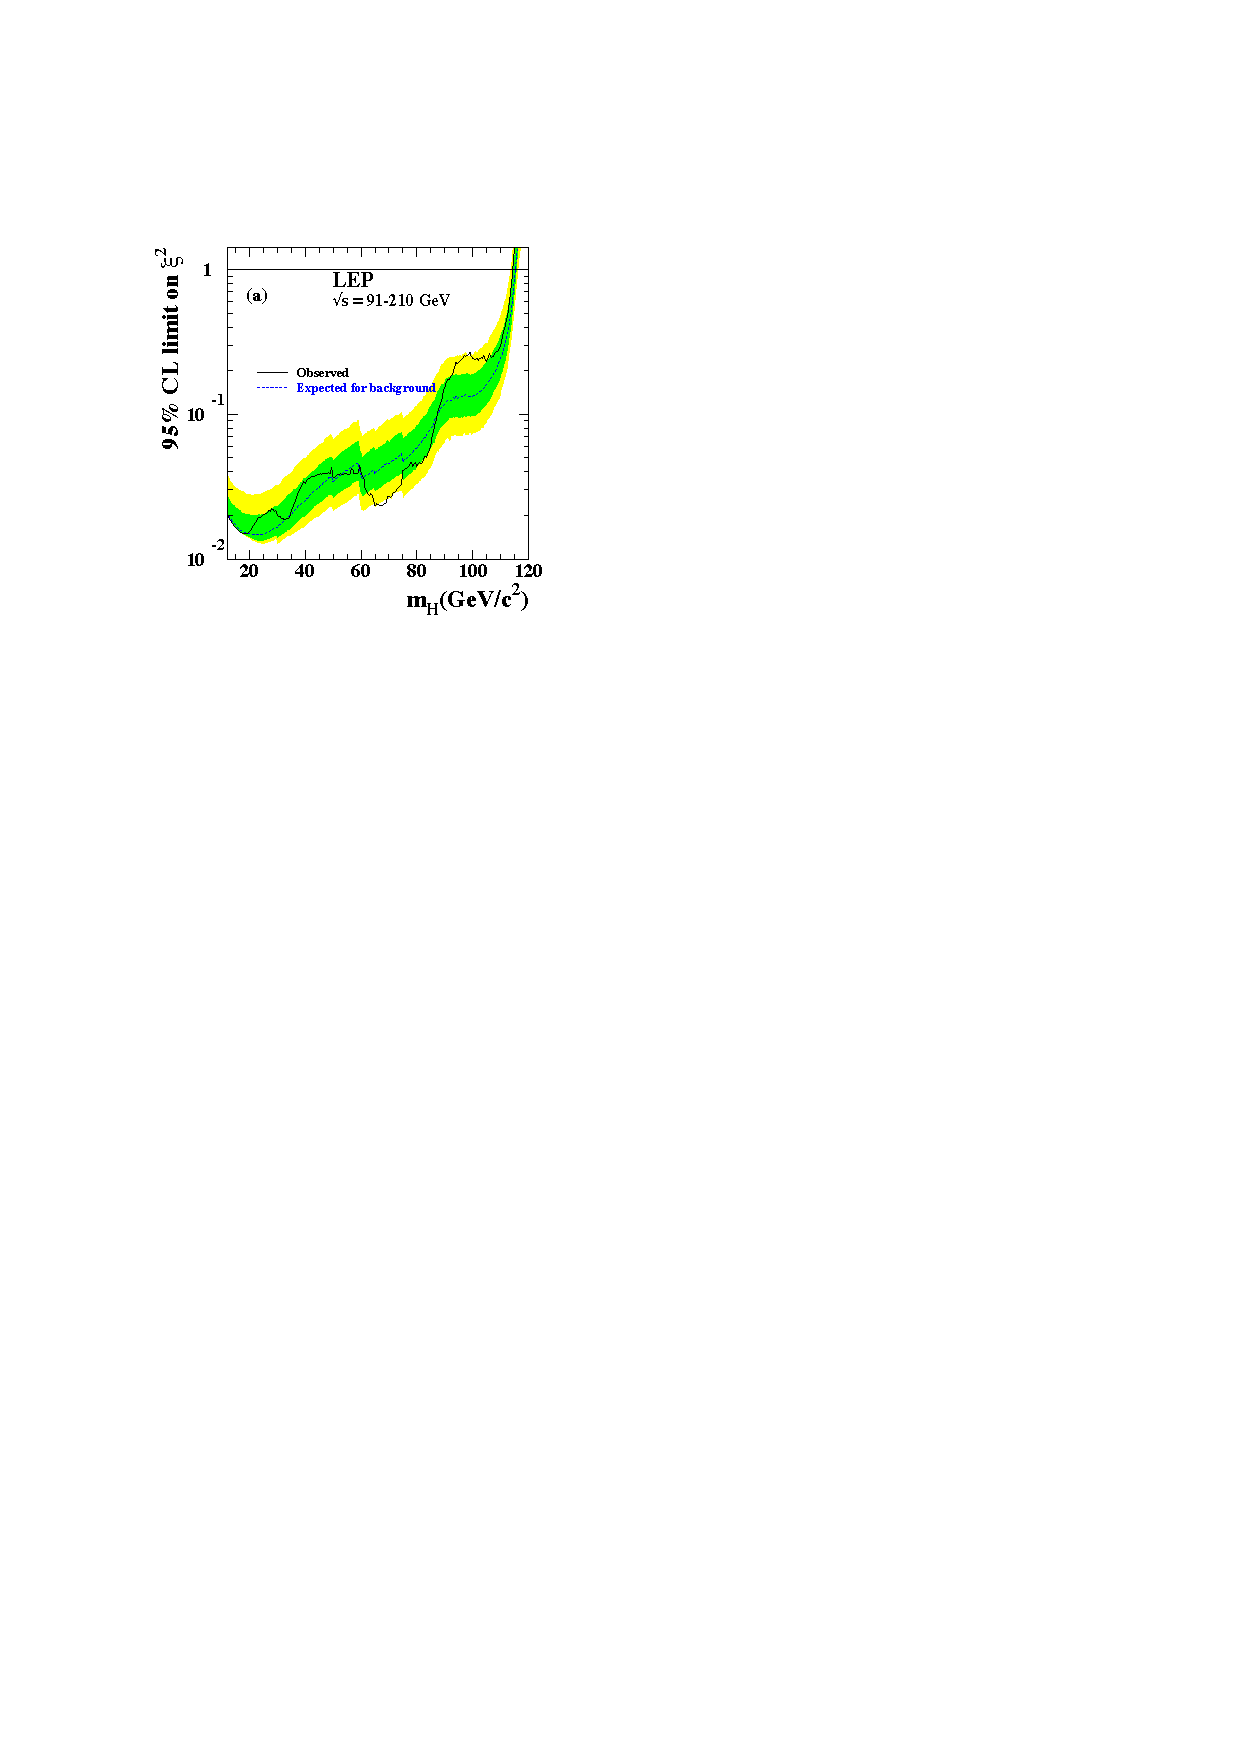
\includegraphics[width=0.47\textwidth]{imagens/lep_exclusion.pdf}
%        }%\hspace{0.1\textwidth}
%        \subfigure[Tevatron, extraído de \cite{tevatron_higgs}.]{%
%            \label{fig:tevatron_exclusion}
%            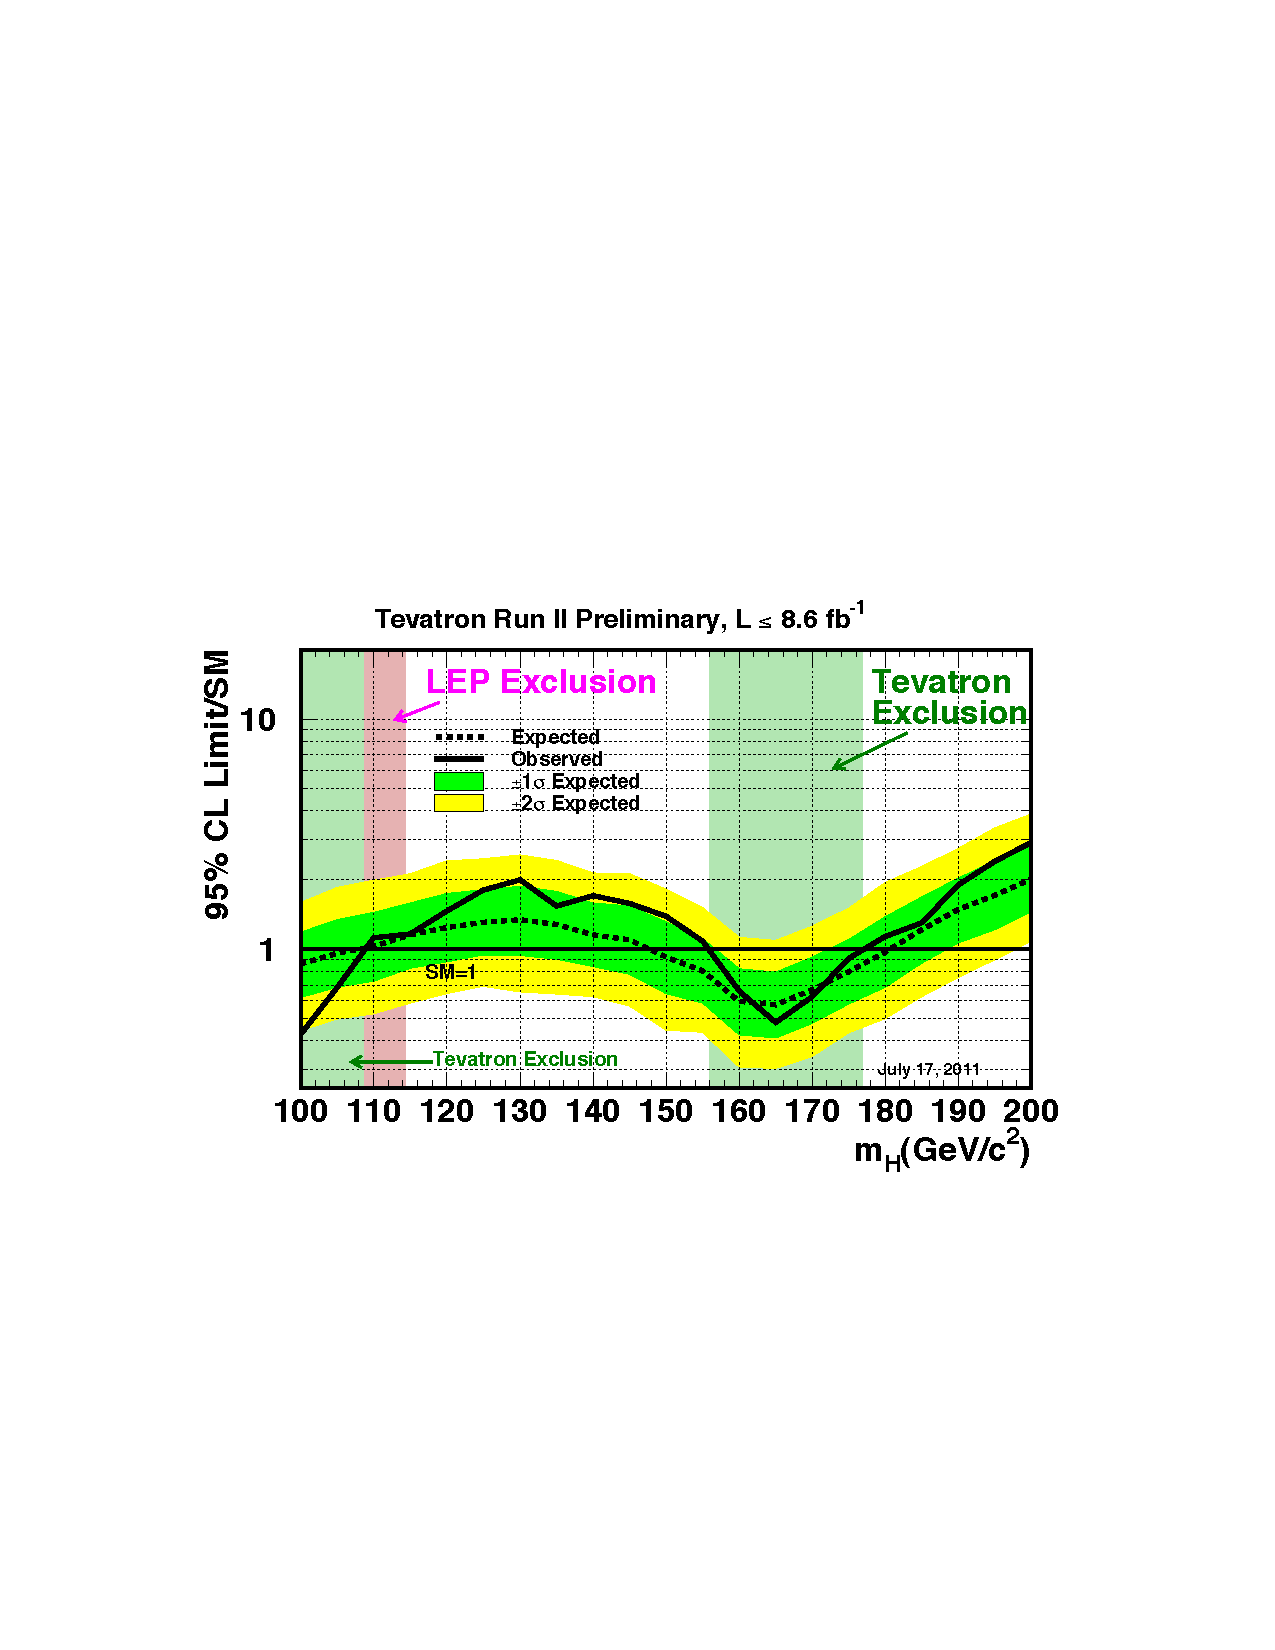
\includegraphics[width=0.47\textwidth]{imagens/tevatron_exclusion.pdf}
%        }\\%\hspace{0.1\textwidth}
%        \subfigure[ATLAS, extraído de \cite{atlas_higgs}.]{
%            \label{fig:atlas_exclusion}
%            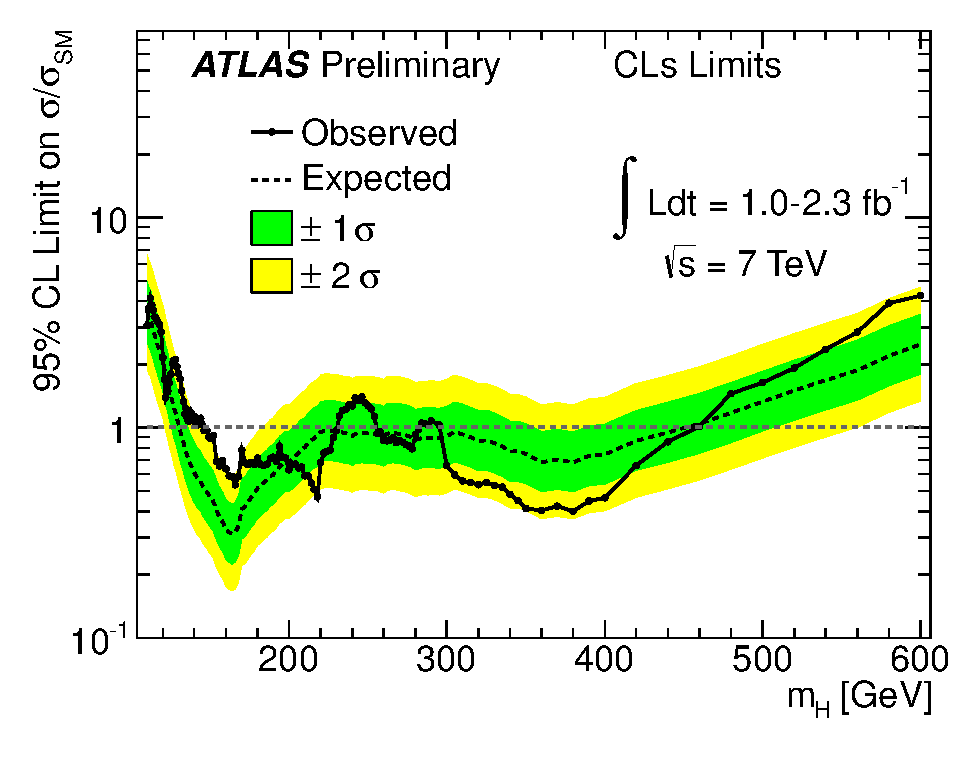
\includegraphics[width=0.47\textwidth]{imagens/atlas_exclusion.pdf}
%        }
%        \subfigure[CMS, extraído de \cite{cms_higgs}.]{%
%            \label{fig:cms_exclusion}
%            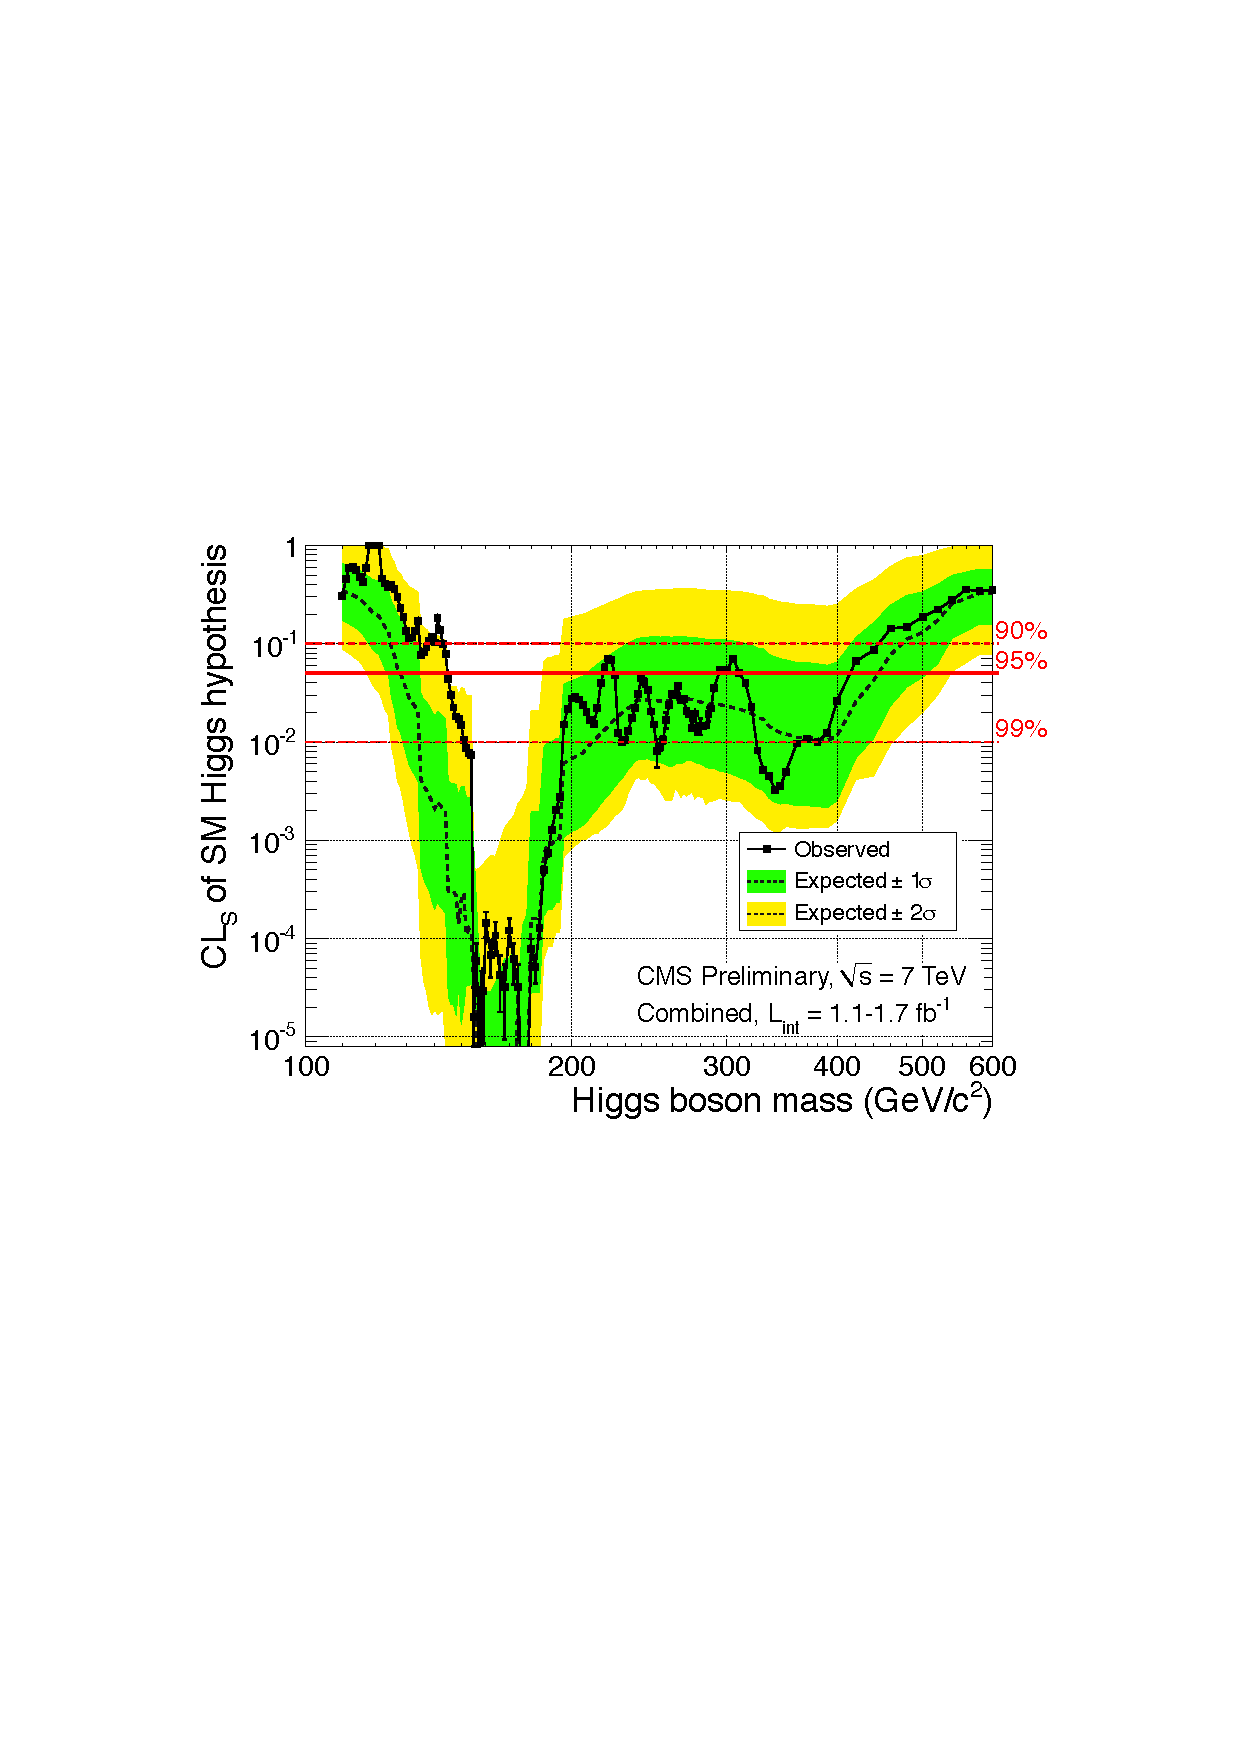
\includegraphics[width=0.47\textwidth]{imagens/cms_exclusion.pdf}
%        }
    \end{center}
\caption[Exclusões de massa do Higgs realizada pela combinação dos dados do
ATLAS e CMS. As exclusões de massa do Tevatron e LEP também estão indicadas.]{As exclusões de massa do bóssom de Higgs. Os valores de massa
observados, no caso para os resultados combinados do ATLAS e CMS, quando
abaixo da linha horizonal vermelha indicada são excluídos com um nível de
confiança de 95\%. A linha pontilhada indica o ruído de fundo esperado gerado
por física na ausência do bóssom de Higgs. As faixas verdes e amarelas indicam
um nível de certeza de 68\% e 95\% de certeza de que algo fora do comum está
ocorrendo. Caso a linha observada ultrapasse o limite superior da faixa amarela
em regiões acima da linha vermelha, então há 95\% de certeza de que há indicios
do bóssom de Higgs ou algum processo de física (talvez ruído físico) não bem
conhecido. Extraído de \cite{atlas_cms_higgs}.}
\end{figure}

Resultados mais recentes excluiram outras regiões de massa do bóssom de Higgs. Em 2008, 
o legado deixado pelo \gls{lep} elevou o limite inferior para 114 GeV/$c^2$
\cite{lep_higgs_2008}, enquanto o experimento Tevatron realizado pelo Fermilab, excluiu as
regiões de $156 < \gls{mh} < 177$ GeV/$c^2$, em Setembro de 2011
\cite{tevatron_higgs}. Também no final de Setembro, resultados preliminares do
\gls{atlas} excluiram o bóssom de Higgs para as regiões de 146-230 GeV/$c^2$, 256-282 GeV/$c^2$ 
e 296-459 GeV/$c^2$ \cite{atlas_higgs}. Um mês antes o \gls{cms} havia excluido o bóssom para
as regiões parecidas: de 145-216 GeV/$c^2$, 226-288 GeV/$c^2$ e 310-400 GeV/$c^2$
\cite{cms_higgs}. Em meados de Novembro o \gls{atlas} e \gls{cms} uniram seus
dados para excluir a região de 141-476 GeV/$c^2$ \cite{atlas_cms_higgs}. Esses
resultados estão indicados na Figura~\ref{fig:higgs_exclusion}, onde estão os
resultados mais recentes do \gls{lhc}, incluidas das regiões anteriormente
excluídas por outros experimentos.


\section{O Sistema de Filtragem (SF)}
\label{sec:sf}

\newacronym[type=Abrev]{asic}{ASIC}{Circuitos Integrados de Aplicação Específica}

O \gls{atlas}, para a luminosidade na qual tem operado: $\sim10^{33}cm^{-2}s^{-1}$,
gera cerca de 19 colisões inelásticas para cada cruzamento entre
feixes, que irão se cruzar numa frequência máxima de 40 MHz. O propósito do
\gls{sf} \cite{trigger_perf_2010,trigger_tdr} é de reduzir essa taxa a cerca
de 200 Hz para seu armazenamento e processamento a posteriori. Esse
limite, correspondendo uma média de $\sim$300 MB/s, é determinado pelos recursos
computacionais para armazenamento e processamento dos dados. É possível gravar
dados com taxas relativamentes mais altas por períodos mais curtos, como foi
realizado durante 2010 quando a física foi beneficiada utilizando taxas de saída
de até $\sim$600 Hz. Nessa época, a luminosidade instantânea máxima atingida foi de
$\sim10^{32}cm^{-2}s^{-1}$, gerando cerca de $\sim$ 1,3 MB, e o \gls{lhc} não 
operava de forma continua -- o que é comum para uma máquina nova -- permitindo 
elevar a taxa de armazenamento.

\newacronym[type=Abrev]{rob}{ROB}{\emph{Buffer} de Leitura}
\newacronym[type=Abrev]{ros}{ROS}{Sistemas de Leitura}

O \gls{sf}, Figura~\ref{fig:sf_esboco}, é dividido em três níveis sequenciais,
sendo descrito aqui resumidamente uma vez que já foi explicada em maiores detalhes em
trabalhos anteriores como \cite{tese_eduardo,tese_torres}, também podendo ser encontrada 
em detalhes nas referências \cite{trigger_tdr,l1_trigger_tdr,l2_ef_daq_dcs_tdr,trigger_perfomance}.

Os sinais do detector são armazenados em memórias \emph{pipeline}, com pendência
à decisão do \acrshort{l1}. Para obter uma latência de menos de 2,5 $\mu$s, 
o \gls{l1} é implementado em rápida eletrônica constituída de \gls{fpga} e
\gls{asic}, de forma a reduzir a taxa para uma valor máximo de 75 kHz. Além do
primeiro passo de seleção, o \gls{l1} identifica as \glspl{roi} do detector a
serem investigadas pelo \acrshort{hlt}. 

\begin{figure}[ht!]
\label{fig:sf_esboco}
\centering
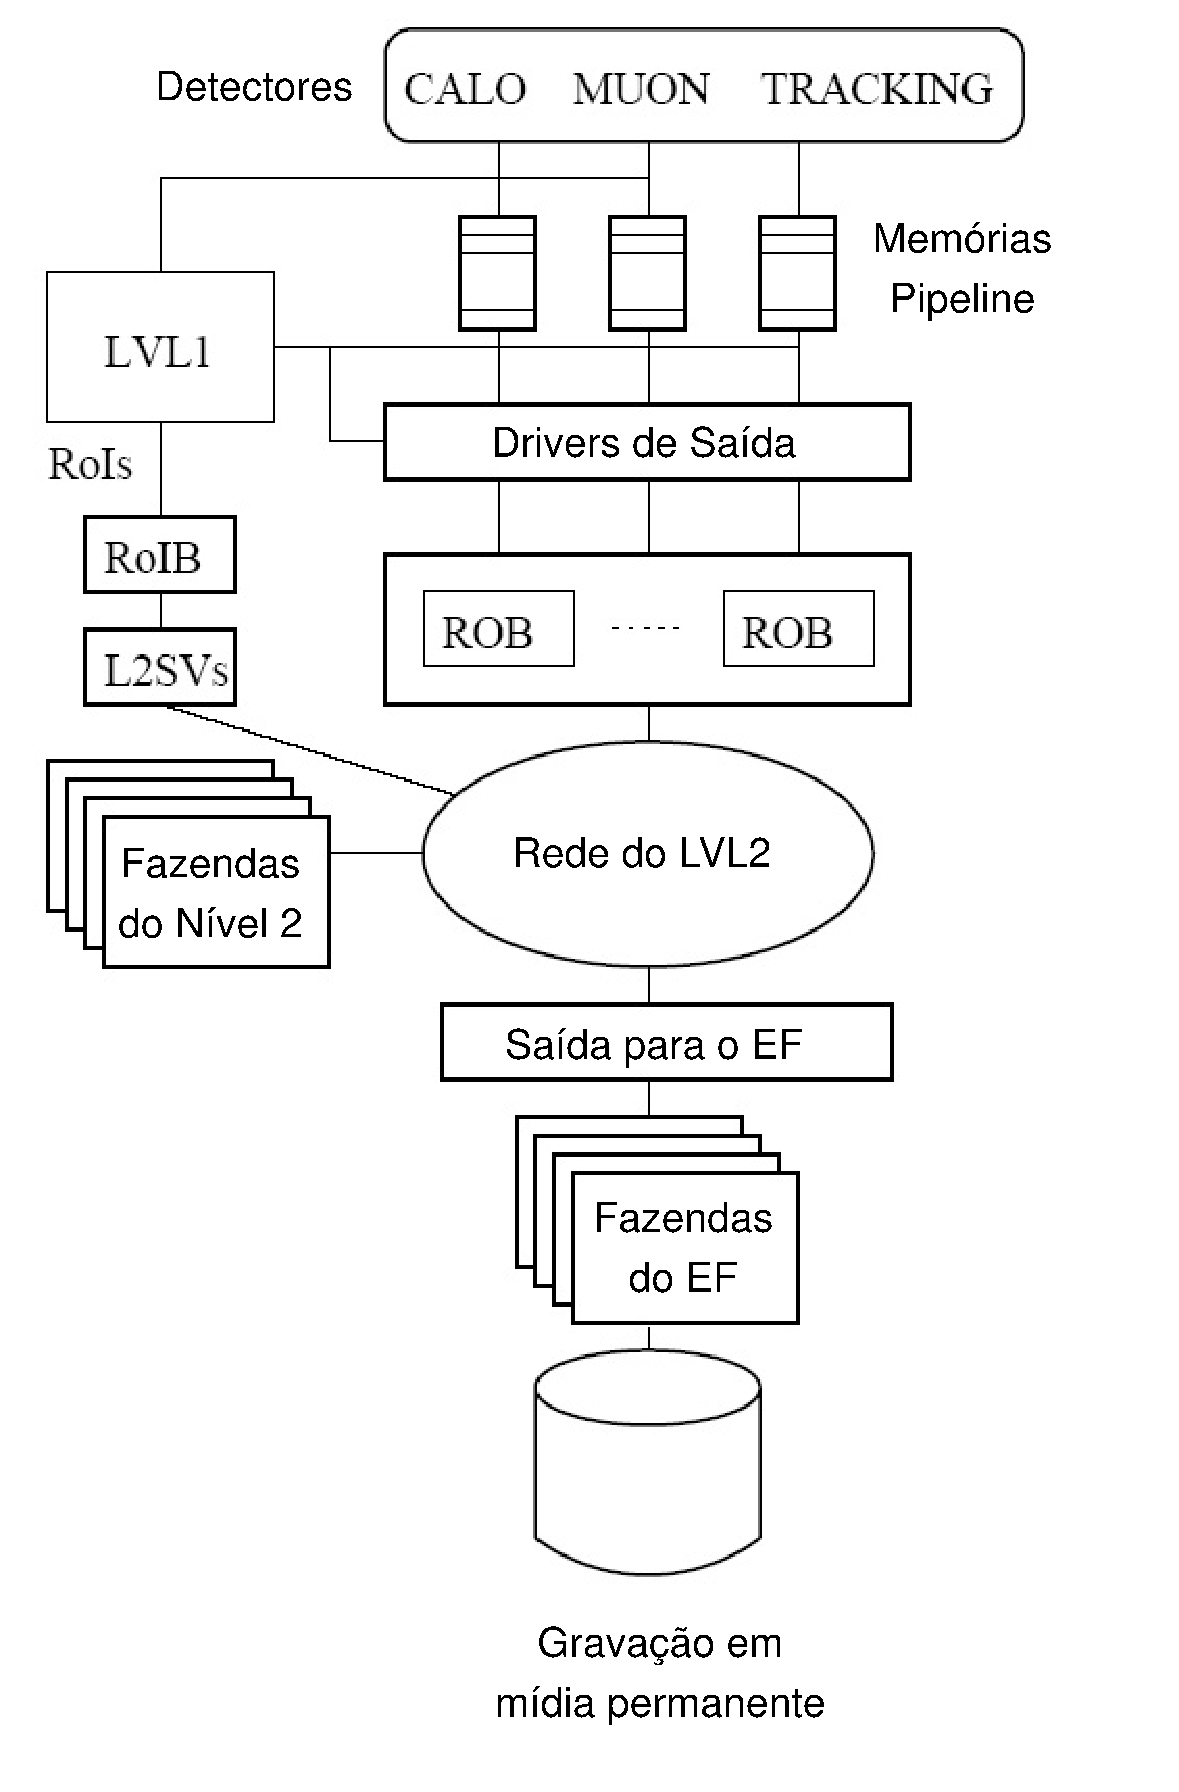
\includegraphics[width=0.6\textwidth]{imagens/sf_resumo.pdf}
\caption[Esboço do Sistema de Filtragem.]{Esboço do Sistema de Filtragem. Extraído de \cite{tese_eduardo}.}
\end{figure}

O \gls{hlt} se consiste de fazendas de
processadores comerciais conectados a rede dedicadas (\emph{Ethernet} de \emph{Gigabit} 
e 10 \emph{Gigabit}).  O \gls{sf} foi projetado para conter cerca de 500 nós para o
\acrshort{l2} e 1800 nós para o \acrshort{ef}\footnote{Em 2010, a fazenda de processamento 
se consistia de 800 nós configuraveis como tanto \acrshort{l2} ou \acrshort{ef}, este 
contendo mais 300 nós dedicados.}. Quando um evento é aceito pelo
\gls{l1}, os dados na memória de cada um dos detectores são então transferidos
para \gls{rob} específicos para cada um dos subdetectores, que armazenam o
evento em fragmentos pendendo à decisão do \gls{l2}. Um ou mais \glspl{rob} são
agrupados para formar os \gls{ros} que são conectados a rede do \gls{hlt}. O
seleção do \gls{l2} é baseada em algoritmos personalizados e rápidos que
processam os dados dos eventos de forma parcial nas regiões especificadas pelas
\glspl{roi} identificadas pelo \gls{l1}. Os processores do \gls{l2} solicitam os
dados dos \gls{ros} correspondentes aelementos do subdetector dentro de cada
\gls{roi}, reduzindo a quantidade de dados a serem transferidas e processadas no
mesmo a cerca de 2-6\% do volume total dos dados. O \gls{l2} reduz a taxa de
dados para cerca de $\sim$3 kHz com uma média de processamento de $\sim$40
ms/evento. Qualquer evento com tempo excedendo a 5 s nesse nível é perdido a
rotulado como evento excedente ao tempo limite.   

O \gls{ef} reune todos os framentos dos eventos aceitos pelo \gls{l2} das
\glspl{rob}, tendo assim acesso a toda sua informação. O \gls{ef} é, em grande
maioria, baseado nos algoritmos do \acrlong{sr} rodando em interfaces
personalizadas para o ambiente do \gls{sf}. Esse nível é projetado para reduzir
os dados para $\sim$200 Hz com uma média de processamento de $\sim$4 s/evento.
Qualquer evento com um tempo excedente a 180 s também é rotulado e perdido como
no \gls{l2}. 

Os eventos de dados selecionados pelo \gls{sf} são escritos nos fluxos de dados
inclusivos, baseados no canal de filtragem. Existem quatro canais de dados
primários: Egamma, Muons, JetTauEtMiss, Minbias, adicionados de diversos canais
de calibração. Cerca de 10\% dos eventos são escritos para um canal expresso
aonde a reconstrução pronta dos eventos é realizada, como foi dito na
Subseção~\ref{ssec:lcg}. Ainda, além da gravação de evnetos completos em um
canal, é possível escrever informação parcial de um ou mais subdetectores em um
canal, o que é normalmente realizado para a calibração do detector nos canais
destinados a esse propósito.

\newacronym[type=Abrev,\glslongpluralkey={Algoritmos de Extração de
Características}]{fex}{FEX}{Algoritmo de Extração de Característica}
\newacronym[type=Abrev,\glslongpluralkey={Algoritmos de Hipótese}]
{hypo}{HYPO}{Algoritmo de Hipótese}

A configuração do \gls{sf} é realizada por um \emph{menu}, que define as
\emph{cadeias} de filtragem que especificam uma sequência de passos de reconstrução e
seleção para as especificas assinaturas de filtragems requeridas pela filtragem.
A cadeia de filtragem de elétrons é ilustrada na Figura~\ref{fig:electron_chain}.
Cada \emph{cadeia} é composta por \gls{fex} que criam objetos,
como os aglomerados de células e variáveis que permitam obter uma informação
sobre a descrição do evento, e \gls{hypo} que fazem a discriminação através dos
critérios de seleção nos objetos gerados, como por exemplo a exigência de um
$\gls{pt} > 20$ GeV. As extrações de características realizadas por uma
\emph{cadeia} podem ser reutilizadas por outro cadeia, reduzindo tanto o acesso
a dados como o tempo de processamento do \gls{sf}.

\begin{figure}[ht!]
\label{fig:electron_chain}
\centering
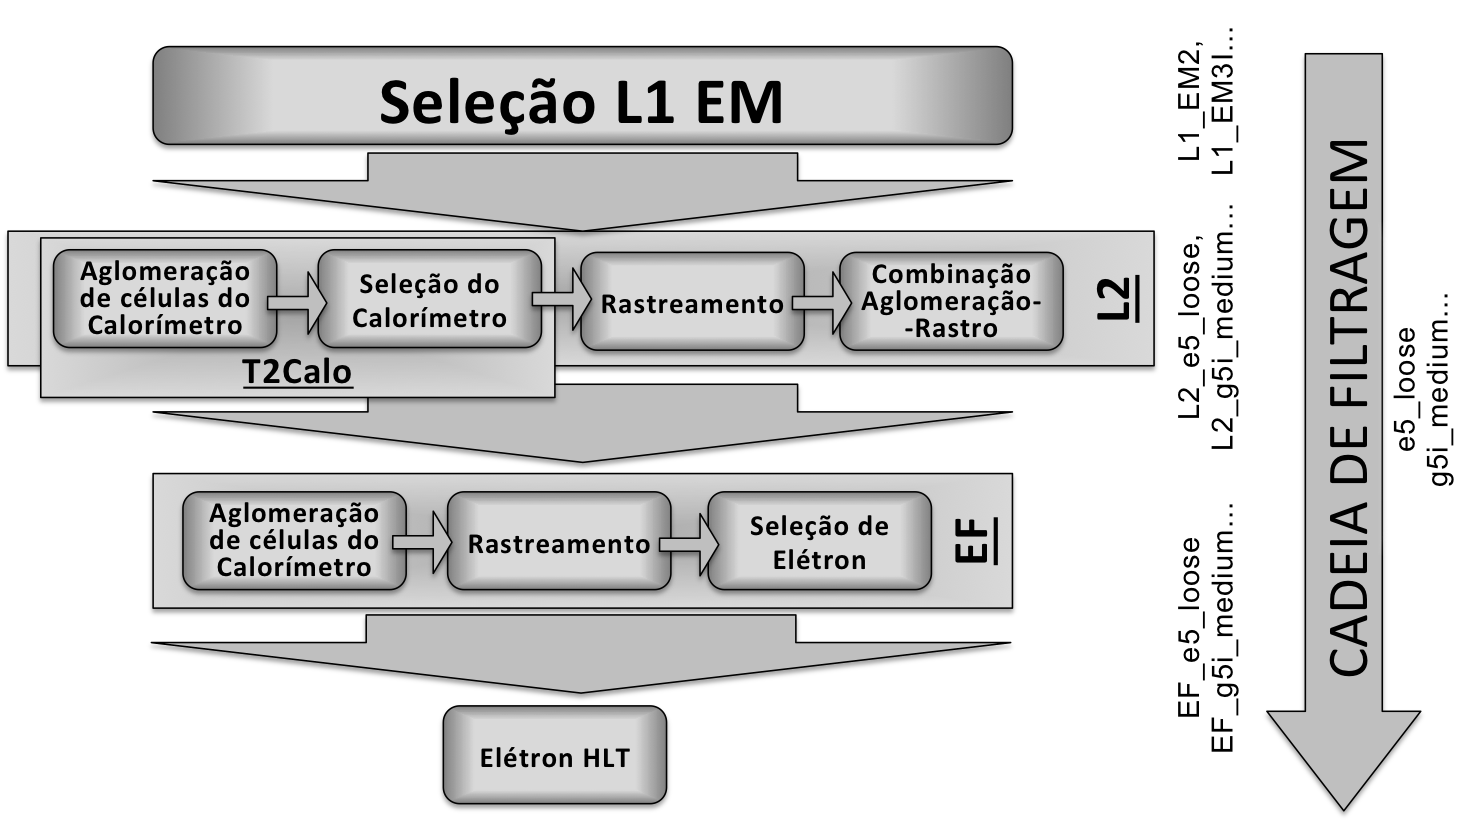
\includegraphics[width=0.9\textwidth]{imagens/cadeia_eletron.png}
\caption[A \emph{cadeia} de filtragem de elétrons.]{A \emph{cadeia} de filtragem
de elétrons. Adaptado de \cite{trigger_perf_2010}.}
\end{figure}

Aproximadamente 500 filtros são definidos nos \emph{menus} atuais, sendo
composto por um número de diferentes classes de filtros:

\begin{enumerate}
\item \textbf{Objetos de filtro único}: usado para determinar estados com pelo
menos um objeto característico. Por exemplo, um filtro para elétron único com um
limiar nominal superior a 3 GeV seria referido como $e3$;
\item \textbf{Objetos de filtro multiplos}: usado para determinar estados finais
com dois ou mais objetos do mesmo tipo. Por exemplo, elétrons duplos decaindo da
partícula $\text{J}/\Psi$. Esses filtros são indicados dependendo de sua
multiplicidade, por exemplo: $2e3$;
\item \textbf{Objetos de filtro combinados}: usados por estados finais de dois
ou mais objetos característicos de tipos diferentes. Por exemplo, um múon de 13
GeV adicionado de 20 GeV de \gls{Etmiss} para selecionar decaimentos
$W\rightarrow \mu\nu$, que seriam denotados de $mu13\_xe20$;
\item \textbf{Filtros Topológicos}: usados para estados finais selecionados de
duas ou mais \glspl{roi}, como no caso do decaimento da partícula
$\text{J}/\Psi$, que combina os traços das duas \glspl{roi} provenientes dos
elétrons.
\end{enumerate}

Quando se referindo a um nível em partícular, o nível (\gls{l1}, \gls{l2},
\gls{ef}) aparece como um prefixo, como por exemplo L1\_EM3 (aqui elétrons e
fótons não são diferenciados, então utiliza-se o prefixo EM em ambos os casos)
para denotar um filtro de elétrons e fótons com um limiar nominal superior a 3
GeV para o \gls{l1} e L2\_e3 no caso de elétrons para um filtro com o mesmo
limiar mas para elétrons apenas no \gls{l2}. Um nome sem o prefixo de nível
refere-se a toda a \emph{cadeia}.

O controle das taxas de filtragem podem ser realizadas mudando os limiares ou
aplicando outros valores de seleção. A seletividade de um grupo de cortes
aplicados para um certo objeto de filtragem é representado pelos termos
\emph{loose} (frouxo), \emph{medium} (mediano), \emph{tight} (apertado). Esses
critérios de seleção são colocados como sufixos ao nome do filtro, por exemplo,
e10\_medium. Requerimentos adicionais como isolamento, podem ser adicionados
para reduzir as taxas dos filtros. O isolamento mede a quantidade de energia, ou
o número de partículas próximos a uma assinatura, se esse valor estiver acima de
um limiar, então a partícula não está isolada. Nesse caso se adiciona a letra
'i' ao nome do filtro, como por exemplo L1\_EM20I ou e20i\_tight.

Fatores de \emph{pré-escala} podem ser adicionados a cada filtro da 
\emph{cadeia} do \gls{hlt}, de tal forma que apenas 1 em cada N eventos passando
o filtro causam que o evento seja aceito por aquele nível. A \emph{pré-escala}
controla a taxa e composição dos canais expressos. Uma série de
\emph{pré-escalas} são utilizadas baseadas em diversas regras que levam em
consideração a prioridade dos filtros em relação com as seguintes categorias:

\begin{enumerate}
\item \textbf{Filtros Primários}: filtros princípais de física, que não deveriam
ser \emph{pré-escalados};
\item \textbf{Filtros de Suporte}: filtros importantes de suporte a filtros
primários, como filtros que permitam estudar a eficiência utilizando 
seletividades mais baixas e limiar mais baixo de \gls{Et} \emph{pré-escalados}
para permitir sua gravação em disco, uma vez que a quantidade de dados que
passam esse filtro será maior;
\item \textbf{Filtros de Monitoração e Calibração}: permitindo a coleta de dados
para garantir a operação correta do \gls{sf} e dos subdetetores do \gls{atlas},
incluindo a calibração dos mesmos. 
\end{enumerate}

\newacronym[type=Abrev]{lb}{LB}{Bloco de Luminosidade} 

Esses fatores de \emph{pré-escala} devem ser modificados conforme a queda da
luminosidade durante um preenchimento do \gls{lhc} de forma a garantir a
maximização das taxas utilizadas pelos filtros, enquanto garantindo uma taxa
constante para a monitoração e calibração. Assim, as mesmas podem ser alteradas
em quaisquer momentos de uma temporada, no início de um novo \gls{lb}. Um
\gls{lb} é a unidade fundamental para a medição da luminosidade, cerca de 120 s
em 2010, na qual se considera que a mesma permaneceu constante com o valor
medido.

Flexibilidade adicional é oferecida ao definir \emph{grupos de pacotes}, separando os
filtros para colisões com pacotes emparelhados (compõe as colisões de física
regulares, contendo pacotes de feixes opostos que se encontram no ponto de
colisão simultaneamente), pacotes vazios para estudo de pedestal criado por ruído 
no detector e raios cósmicos, ou até mesmo configurações mais inusitadas, como 
exigindo pacotes desparelhados separados por no mínimo 75 ns de quaisquer outro 
pacote no outro feixe.

\subsection{T2Calo}
\label{ssec:t2calo}

% Falar sobre Fex 
% Colocar rcore, eratio etc, fazendo referencia ao processo de geracao dos
% chuveiros

% Falar sobre Hypo
% cortes lineares, estudados a partir de Monte Carlo

\subsection{HLT\_EgammaCaloRinger (Ringer\_HLT)}
\label{ssec:hlt_ringer}

% Explicar o processo de anelamento

% Falar sobre redes neurais

% Pre-processamento: normalizacao, ica etc

\section{O Sistema de Reconstrução (SR)}
\label{sec:sr}

% Falar aqui que o Sistema de Filtragem é uma versão mais simples do Sistema de
% Reconstrução

\subsection{\texorpdfstring{Algoritmo $e/\gamma$ Padrão}{Algoritmo eGamma Padrão}}
\label{ssec:egamma}


% Falar que tem mais opções que 
% Colocar os requerimentos, tight, loose, medium.


\subsection{\texorpdfstring{$e/\gamma$ \emph{Calorimeter Ringer}
(EgCaloRinger)}{eGamma Calorimeter Ringer (EgCaloRinger)}}
\label{ssec:egringer}

% Falar aqui da request feito pela colaboracao

\subsubsection{Implementação}
\label{sssec:egringer_impl}
% Implementação



